% Created by tikzDevice version 0.12.3.1 on 2023-02-07 16:22:26
% !TEX encoding = UTF-8 Unicode
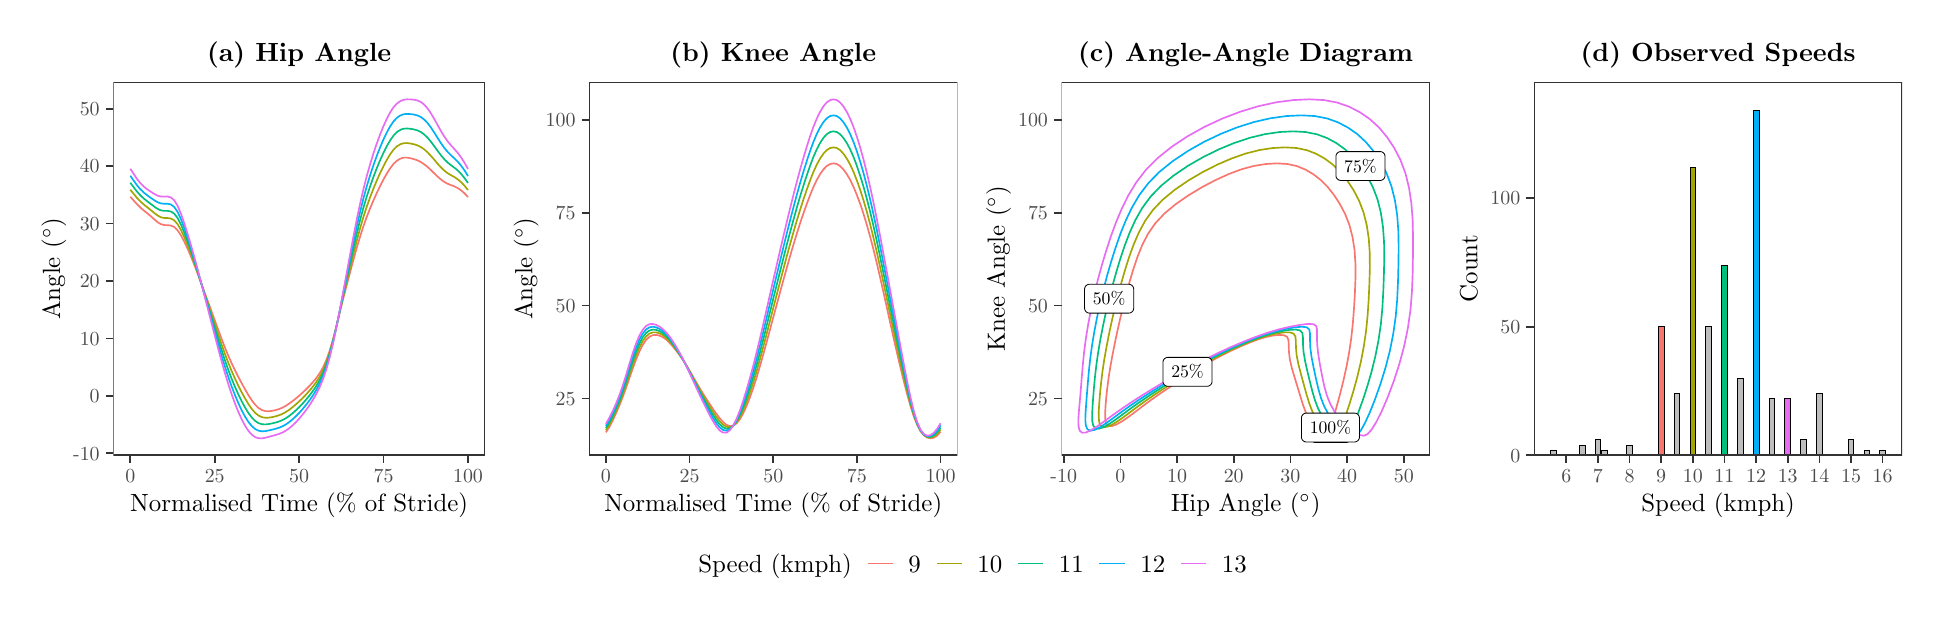
\begin{tikzpicture}[x=1pt,y=1pt]
\definecolor{fillColor}{RGB}{255,255,255}
\path[use as bounding box,fill=fillColor,fill opacity=0.00] (0,0) rectangle (682.86,204.86);
\begin{scope}
\path[clip] (  0.00, 22.44) rectangle (170.72,204.86);
\definecolor{drawColor}{RGB}{255,255,255}
\definecolor{fillColor}{RGB}{255,255,255}

\path[draw=drawColor,line width= 0.6pt,line join=round,line cap=round,fill=fillColor] ( -0.00, 22.44) rectangle (170.72,204.86);
\end{scope}
\begin{scope}
\path[clip] ( 30.98, 50.33) rectangle (165.22,185.10);
\definecolor{fillColor}{RGB}{255,255,255}

\path[fill=fillColor] ( 30.98, 50.33) rectangle (165.22,185.10);
\definecolor{drawColor}{RGB}{248,118,109}

\path[draw=drawColor,line width= 0.6pt,line join=round] ( 37.09,143.77) --
	( 38.31,142.40) --
	( 39.53,141.05) --
	( 40.75,139.85) --
	( 41.97,138.79) --
	( 43.19,137.82) --
	( 44.41,136.81) --
	( 45.63,135.71) --
	( 46.85,134.66) --
	( 48.07,133.88) --
	( 49.29,133.54) --
	( 50.51,133.48) --
	( 51.73,133.36) --
	( 52.95,132.83) --
	( 54.17,131.65) --
	( 55.39,129.81) --
	( 56.61,127.50) --
	( 57.83,124.89) --
	( 59.05,122.08) --
	( 60.27,119.02) --
	( 61.49,115.78) --
	( 62.71,112.45) --
	( 63.93,109.14) --
	( 65.15,105.84) --
	( 66.37,102.51) --
	( 67.59, 99.16) --
	( 68.81, 95.81) --
	( 70.03, 92.50) --
	( 71.25, 89.34) --
	( 72.47, 86.37) --
	( 73.69, 83.62) --
	( 74.91, 81.06) --
	( 76.13, 78.65) --
	( 77.35, 76.34) --
	( 78.58, 74.12) --
	( 79.80, 72.02) --
	( 81.02, 70.14) --
	( 82.24, 68.57) --
	( 83.46, 67.40) --
	( 84.68, 66.66) --
	( 85.90, 66.31) --
	( 87.12, 66.26) --
	( 88.34, 66.40) --
	( 89.56, 66.66) --
	( 90.78, 67.03) --
	( 92.00, 67.53) --
	( 93.22, 68.18) --
	( 94.44, 68.98) --
	( 95.66, 69.87) --
	( 96.88, 70.84) --
	( 98.10, 71.87) --
	( 99.32, 72.97) --
	(100.54, 74.12) --
	(101.76, 75.36) --
	(102.98, 76.69) --
	(104.20, 78.15) --
	(105.42, 79.85) --
	(106.64, 81.92) --
	(107.86, 84.58) --
	(109.08, 87.98) --
	(110.30, 92.12) --
	(111.52, 96.85) --
	(112.74,101.83) --
	(113.96,106.73) --
	(115.18,111.46) --
	(116.40,116.09) --
	(117.62,120.65) --
	(118.84,125.06) --
	(120.07,129.20) --
	(121.29,133.01) --
	(122.51,136.45) --
	(123.73,139.57) --
	(124.95,142.47) --
	(126.17,145.19) --
	(127.39,147.73) --
	(128.61,150.08) --
	(129.83,152.24) --
	(131.05,154.15) --
	(132.27,155.71) --
	(133.49,156.84) --
	(134.71,157.56) --
	(135.93,157.89) --
	(137.15,157.89) --
	(138.37,157.67) --
	(139.59,157.35) --
	(140.81,156.92) --
	(142.03,156.33) --
	(143.25,155.53) --
	(144.47,154.55) --
	(145.69,153.43) --
	(146.91,152.23) --
	(148.13,151.05) --
	(149.35,149.98) --
	(150.57,149.10) --
	(151.79,148.43) --
	(153.01,147.94) --
	(154.23,147.49) --
	(155.45,146.88) --
	(156.67,146.03) --
	(157.89,144.95) --
	(159.11,143.66);
\definecolor{drawColor}{RGB}{163,165,0}

\path[draw=drawColor,line width= 0.6pt,line join=round] ( 37.09,146.30) --
	( 38.31,144.79) --
	( 39.53,143.33) --
	( 40.75,142.05) --
	( 41.97,140.95) --
	( 43.19,139.98) --
	( 44.41,139.01) --
	( 45.63,138.00) --
	( 46.85,137.05) --
	( 48.07,136.37) --
	( 49.29,136.10) --
	( 50.51,136.07) --
	( 51.73,135.90) --
	( 52.95,135.25) --
	( 54.17,133.86) --
	( 55.39,131.76) --
	( 56.61,129.14) --
	( 57.83,126.22) --
	( 59.05,123.08) --
	( 60.27,119.70) --
	( 61.49,116.14) --
	( 62.71,112.49) --
	( 63.93,108.83) --
	( 65.15,105.17) --
	( 66.37,101.48) --
	( 67.59, 97.79) --
	( 68.81, 94.10) --
	( 70.03, 90.49) --
	( 71.25, 87.04) --
	( 72.47, 83.82) --
	( 73.69, 80.83) --
	( 74.91, 78.06) --
	( 76.13, 75.49) --
	( 77.35, 73.08) --
	( 78.58, 70.83) --
	( 79.80, 68.79) --
	( 81.02, 67.04) --
	( 82.24, 65.65) --
	( 83.46, 64.67) --
	( 84.68, 64.11) --
	( 85.90, 63.90) --
	( 87.12, 63.94) --
	( 88.34, 64.13) --
	( 89.56, 64.41) --
	( 90.78, 64.78) --
	( 92.00, 65.28) --
	( 93.22, 65.94) --
	( 94.44, 66.74) --
	( 95.66, 67.67) --
	( 96.88, 68.69) --
	( 98.10, 69.80) --
	( 99.32, 70.98) --
	(100.54, 72.25) --
	(101.76, 73.60) --
	(102.98, 75.07) --
	(104.20, 76.70) --
	(105.42, 78.58) --
	(106.64, 80.86) --
	(107.86, 83.74) --
	(109.08, 87.36) --
	(110.30, 91.75) --
	(111.52, 96.74) --
	(112.74,102.04) --
	(113.96,107.33) --
	(115.18,112.52) --
	(116.40,117.65) --
	(117.62,122.71) --
	(118.84,127.59) --
	(120.07,132.16) --
	(121.29,136.35) --
	(122.51,140.13) --
	(123.73,143.55) --
	(124.95,146.71) --
	(126.17,149.66) --
	(127.39,152.39) --
	(128.61,154.90) --
	(129.83,157.19) --
	(131.05,159.20) --
	(132.27,160.83) --
	(133.49,162.01) --
	(134.71,162.76) --
	(135.93,163.12) --
	(137.15,163.16) --
	(138.37,162.99) --
	(139.59,162.72) --
	(140.81,162.34) --
	(142.03,161.76) --
	(143.25,160.92) --
	(144.47,159.84) --
	(145.69,158.56) --
	(146.91,157.15) --
	(148.13,155.71) --
	(149.35,154.36) --
	(150.57,153.19) --
	(151.79,152.26) --
	(153.01,151.53) --
	(154.23,150.86) --
	(155.45,150.04) --
	(156.67,148.99) --
	(157.89,147.70) --
	(159.11,146.19);
\definecolor{drawColor}{RGB}{0,191,125}

\path[draw=drawColor,line width= 0.6pt,line join=round] ( 37.09,148.83) --
	( 38.31,147.18) --
	( 39.53,145.61) --
	( 40.75,144.25) --
	( 41.97,143.11) --
	( 43.19,142.14) --
	( 44.41,141.22) --
	( 45.63,140.29) --
	( 46.85,139.44) --
	( 48.07,138.87) --
	( 49.29,138.67) --
	( 50.51,138.66) --
	( 51.73,138.44) --
	( 52.95,137.66) --
	( 54.17,136.08) --
	( 55.39,133.72) --
	( 56.61,130.79) --
	( 57.83,127.54) --
	( 59.05,124.08) --
	( 60.27,120.39) --
	( 61.49,116.50) --
	( 62.71,112.52) --
	( 63.93,108.51) --
	( 65.15,104.49) --
	( 66.37,100.46) --
	( 67.59, 96.41) --
	( 68.81, 92.40) --
	( 70.03, 88.48) --
	( 71.25, 84.75) --
	( 72.47, 81.26) --
	( 73.69, 78.03) --
	( 74.91, 75.06) --
	( 76.13, 72.33) --
	( 77.35, 69.82) --
	( 78.58, 67.55) --
	( 79.80, 65.57) --
	( 81.02, 63.95) --
	( 82.24, 62.73) --
	( 83.46, 61.94) --
	( 84.68, 61.56) --
	( 85.90, 61.50) --
	( 87.12, 61.63) --
	( 88.34, 61.87) --
	( 89.56, 62.16) --
	( 90.78, 62.53) --
	( 92.00, 63.03) --
	( 93.22, 63.69) --
	( 94.44, 64.51) --
	( 95.66, 65.47) --
	( 96.88, 66.55) --
	( 98.10, 67.72) --
	( 99.32, 69.00) --
	(100.54, 70.37) --
	(101.76, 71.84) --
	(102.98, 73.45) --
	(104.20, 75.24) --
	(105.42, 77.31) --
	(106.64, 79.79) --
	(107.86, 82.89) --
	(109.08, 86.74) --
	(110.30, 91.37) --
	(111.52, 96.63) --
	(112.74,102.25) --
	(113.96,107.94) --
	(115.18,113.58) --
	(116.40,119.20) --
	(117.62,124.77) --
	(118.84,130.12) --
	(120.07,135.13) --
	(121.29,139.69) --
	(122.51,143.81) --
	(123.73,147.52) --
	(124.95,150.94) --
	(126.17,154.13) --
	(127.39,157.06) --
	(128.61,159.73) --
	(129.83,162.15) --
	(131.05,164.25) --
	(132.27,165.95) --
	(133.49,167.17) --
	(134.71,167.96) --
	(135.93,168.36) --
	(137.15,168.43) --
	(138.37,168.30) --
	(139.59,168.09) --
	(140.81,167.75) --
	(142.03,167.18) --
	(143.25,166.31) --
	(144.47,165.13) --
	(145.69,163.69) --
	(146.91,162.06) --
	(148.13,160.36) --
	(149.35,158.74) --
	(150.57,157.29) --
	(151.79,156.09) --
	(153.01,155.12) --
	(154.23,154.23) --
	(155.45,153.21) --
	(156.67,151.96) --
	(157.89,150.46) --
	(159.11,148.73);
\definecolor{drawColor}{RGB}{0,176,246}

\path[draw=drawColor,line width= 0.6pt,line join=round] ( 37.09,151.36) --
	( 38.31,149.58) --
	( 39.53,147.88) --
	( 40.75,146.45) --
	( 41.97,145.27) --
	( 43.19,144.30) --
	( 44.41,143.42) --
	( 45.63,142.57) --
	( 46.85,141.83) --
	( 48.07,141.36) --
	( 49.29,141.24) --
	( 50.51,141.25) --
	( 51.73,140.98) --
	( 52.95,140.07) --
	( 54.17,138.29) --
	( 55.39,135.67) --
	( 56.61,132.44) --
	( 57.83,128.87) --
	( 59.05,125.09) --
	( 60.27,121.07) --
	( 61.49,116.86) --
	( 62.71,112.55) --
	( 63.93,108.20) --
	( 65.15,103.82) --
	( 66.37, 99.43) --
	( 67.59, 95.04) --
	( 68.81, 90.70) --
	( 70.03, 86.48) --
	( 71.25, 82.46) --
	( 72.47, 78.70) --
	( 73.69, 75.24) --
	( 74.91, 72.06) --
	( 76.13, 69.17) --
	( 77.35, 66.56) --
	( 78.58, 64.27) --
	( 79.80, 62.34) --
	( 81.02, 60.85) --
	( 82.24, 59.81) --
	( 83.46, 59.21) --
	( 84.68, 59.01) --
	( 85.90, 59.09) --
	( 87.12, 59.32) --
	( 88.34, 59.60) --
	( 89.56, 59.92) --
	( 90.78, 60.29) --
	( 92.00, 60.78) --
	( 93.22, 61.44) --
	( 94.44, 62.28) --
	( 95.66, 63.28) --
	( 96.88, 64.40) --
	( 98.10, 65.65) --
	( 99.32, 67.01) --
	(100.54, 68.49) --
	(101.76, 70.08) --
	(102.98, 71.83) --
	(104.20, 73.78) --
	(105.42, 76.04) --
	(106.64, 78.73) --
	(107.86, 82.05) --
	(109.08, 86.12) --
	(110.30, 90.99) --
	(111.52, 96.52) --
	(112.74,102.46) --
	(113.96,108.54) --
	(115.18,114.64) --
	(116.40,120.76) --
	(117.62,126.82) --
	(118.84,132.65) --
	(120.07,138.09) --
	(121.29,143.04) --
	(122.51,147.49) --
	(123.73,151.50) --
	(124.95,155.18) --
	(126.17,158.59) --
	(127.39,161.73) --
	(128.61,164.56) --
	(129.83,167.10) --
	(131.05,169.30) --
	(132.27,171.07) --
	(133.49,172.34) --
	(134.71,173.16) --
	(135.93,173.59) --
	(137.15,173.70) --
	(138.37,173.62) --
	(139.59,173.46) --
	(140.81,173.16) --
	(142.03,172.61) --
	(143.25,171.70) --
	(144.47,170.43) --
	(145.69,168.82) --
	(146.91,166.97) --
	(148.13,165.01) --
	(149.35,163.11) --
	(150.57,161.39) --
	(151.79,159.92) --
	(153.01,158.70) --
	(154.23,157.59) --
	(155.45,156.38) --
	(156.67,154.93) --
	(157.89,153.22) --
	(159.11,151.26);
\definecolor{drawColor}{RGB}{231,107,243}

\path[draw=drawColor,line width= 0.6pt,line join=round] ( 37.09,153.89) --
	( 38.31,151.97) --
	( 39.53,150.16) --
	( 40.75,148.64) --
	( 41.97,147.42) --
	( 43.19,146.46) --
	( 44.41,145.63) --
	( 45.63,144.86) --
	( 46.85,144.21) --
	( 48.07,143.85) --
	( 49.29,143.81) --
	( 50.51,143.84) --
	( 51.73,143.52) --
	( 52.95,142.49) --
	( 54.17,140.51) --
	( 55.39,137.62) --
	( 56.61,134.09) --
	( 57.83,130.20) --
	( 59.05,126.09) --
	( 60.27,121.76) --
	( 61.49,117.23) --
	( 62.71,112.58) --
	( 63.93,107.89) --
	( 65.15,103.15) --
	( 66.37, 98.40) --
	( 67.59, 93.67) --
	( 68.81, 89.00) --
	( 70.03, 84.47) --
	( 71.25, 80.16) --
	( 72.47, 76.15) --
	( 73.69, 72.44) --
	( 74.91, 69.06) --
	( 76.13, 66.01) --
	( 77.35, 63.30) --
	( 78.58, 60.99) --
	( 79.80, 59.12) --
	( 81.02, 57.75) --
	( 82.24, 56.89) --
	( 83.46, 56.48) --
	( 84.68, 56.46) --
	( 85.90, 56.68) --
	( 87.12, 57.00) --
	( 88.34, 57.34) --
	( 89.56, 57.67) --
	( 90.78, 58.04) --
	( 92.00, 58.53) --
	( 93.22, 59.19) --
	( 94.44, 60.05) --
	( 95.66, 61.08) --
	( 96.88, 62.25) --
	( 98.10, 63.58) --
	( 99.32, 65.03) --
	(100.54, 66.61) --
	(101.76, 68.32) --
	(102.98, 70.21) --
	(104.20, 72.33) --
	(105.42, 74.76) --
	(106.64, 77.66) --
	(107.86, 81.20) --
	(109.08, 85.51) --
	(110.30, 90.61) --
	(111.52, 96.41) --
	(112.74,102.67) --
	(113.96,109.14) --
	(115.18,115.70) --
	(116.40,122.31) --
	(117.62,128.88) --
	(118.84,135.18) --
	(120.07,141.05) --
	(121.29,146.38) --
	(122.51,151.17) --
	(123.73,155.47) --
	(124.95,159.42) --
	(126.17,163.06) --
	(127.39,166.39) --
	(128.61,169.38) --
	(129.83,172.05) --
	(131.05,174.35) --
	(132.27,176.19) --
	(133.49,177.50) --
	(134.71,178.36) --
	(135.93,178.82) --
	(137.15,178.97) --
	(138.37,178.94) --
	(139.59,178.83) --
	(140.81,178.58) --
	(142.03,178.04) --
	(143.25,177.09) --
	(144.47,175.72) --
	(145.69,173.95) --
	(146.91,171.88) --
	(148.13,169.67) --
	(149.35,167.49) --
	(150.57,165.48) --
	(151.79,163.75) --
	(153.01,162.29) --
	(154.23,160.96) --
	(155.45,159.55) --
	(156.67,157.90) --
	(157.89,155.97) --
	(159.11,153.80);
\definecolor{drawColor}{gray}{0.20}

\path[draw=drawColor,line width= 0.6pt,line join=round,line cap=round] ( 30.98, 50.33) rectangle (165.22,185.10);
\end{scope}
\begin{scope}
\path[clip] (  0.00,  0.00) rectangle (682.86,204.86);
\definecolor{drawColor}{gray}{0.30}

\node[text=drawColor,anchor=base east,inner sep=0pt, outer sep=0pt, scale=  0.72] at ( 26.03, 48.62) {-10};

\node[text=drawColor,anchor=base east,inner sep=0pt, outer sep=0pt, scale=  0.72] at ( 26.03, 69.37) {0};

\node[text=drawColor,anchor=base east,inner sep=0pt, outer sep=0pt, scale=  0.72] at ( 26.03, 90.11) {10};

\node[text=drawColor,anchor=base east,inner sep=0pt, outer sep=0pt, scale=  0.72] at ( 26.03,110.86) {20};

\node[text=drawColor,anchor=base east,inner sep=0pt, outer sep=0pt, scale=  0.72] at ( 26.03,131.60) {30};

\node[text=drawColor,anchor=base east,inner sep=0pt, outer sep=0pt, scale=  0.72] at ( 26.03,152.35) {40};

\node[text=drawColor,anchor=base east,inner sep=0pt, outer sep=0pt, scale=  0.72] at ( 26.03,173.09) {50};
\end{scope}
\begin{scope}
\path[clip] (  0.00,  0.00) rectangle (682.86,204.86);
\definecolor{drawColor}{gray}{0.20}

\path[draw=drawColor,line width= 0.6pt,line join=round] ( 28.23, 51.10) --
	( 30.98, 51.10);

\path[draw=drawColor,line width= 0.6pt,line join=round] ( 28.23, 71.84) --
	( 30.98, 71.84);

\path[draw=drawColor,line width= 0.6pt,line join=round] ( 28.23, 92.59) --
	( 30.98, 92.59);

\path[draw=drawColor,line width= 0.6pt,line join=round] ( 28.23,113.34) --
	( 30.98,113.34);

\path[draw=drawColor,line width= 0.6pt,line join=round] ( 28.23,134.08) --
	( 30.98,134.08);

\path[draw=drawColor,line width= 0.6pt,line join=round] ( 28.23,154.83) --
	( 30.98,154.83);

\path[draw=drawColor,line width= 0.6pt,line join=round] ( 28.23,175.57) --
	( 30.98,175.57);
\end{scope}
\begin{scope}
\path[clip] (  0.00,  0.00) rectangle (682.86,204.86);
\definecolor{drawColor}{gray}{0.20}

\path[draw=drawColor,line width= 0.6pt,line join=round] ( 37.09, 47.58) --
	( 37.09, 50.33);

\path[draw=drawColor,line width= 0.6pt,line join=round] ( 67.59, 47.58) --
	( 67.59, 50.33);

\path[draw=drawColor,line width= 0.6pt,line join=round] ( 98.10, 47.58) --
	( 98.10, 50.33);

\path[draw=drawColor,line width= 0.6pt,line join=round] (128.61, 47.58) --
	(128.61, 50.33);

\path[draw=drawColor,line width= 0.6pt,line join=round] (159.11, 47.58) --
	(159.11, 50.33);
\end{scope}
\begin{scope}
\path[clip] (  0.00,  0.00) rectangle (682.86,204.86);
\definecolor{drawColor}{gray}{0.30}

\node[text=drawColor,anchor=base,inner sep=0pt, outer sep=0pt, scale=  0.72] at ( 37.09, 40.42) {0};

\node[text=drawColor,anchor=base,inner sep=0pt, outer sep=0pt, scale=  0.72] at ( 67.59, 40.42) {25};

\node[text=drawColor,anchor=base,inner sep=0pt, outer sep=0pt, scale=  0.72] at ( 98.10, 40.42) {50};

\node[text=drawColor,anchor=base,inner sep=0pt, outer sep=0pt, scale=  0.72] at (128.61, 40.42) {75};

\node[text=drawColor,anchor=base,inner sep=0pt, outer sep=0pt, scale=  0.72] at (159.11, 40.42) {100};
\end{scope}
\begin{scope}
\path[clip] (  0.00,  0.00) rectangle (682.86,204.86);
\definecolor{drawColor}{RGB}{0,0,0}

\node[text=drawColor,anchor=base,inner sep=0pt, outer sep=0pt, scale=  0.90] at ( 98.10, 29.93) {Normalised Time ($\%$ of Stride)};
\end{scope}
\begin{scope}
\path[clip] (  0.00,  0.00) rectangle (682.86,204.86);
\definecolor{drawColor}{RGB}{0,0,0}

\node[text=drawColor,rotate= 90.00,anchor=base,inner sep=0pt, outer sep=0pt, scale=  0.90] at ( 11.70,117.71) {Angle ($^{\circ}$)};
\end{scope}
\begin{scope}
\path[clip] (  0.00,  0.00) rectangle (682.86,204.86);
\definecolor{drawColor}{RGB}{0,0,0}

\node[text=drawColor,anchor=base,inner sep=0pt, outer sep=0pt, scale=  0.95] at ( 98.10,192.80) {\bfseries (a) Hip Angle};
\end{scope}
\begin{scope}
\path[clip] (170.72, 22.44) rectangle (341.43,204.86);
\definecolor{drawColor}{RGB}{255,255,255}
\definecolor{fillColor}{RGB}{255,255,255}

\path[draw=drawColor,line width= 0.6pt,line join=round,line cap=round,fill=fillColor] (170.72, 22.44) rectangle (341.43,204.86);
\end{scope}
\begin{scope}
\path[clip] (202.90, 50.33) rectangle (335.93,185.10);
\definecolor{fillColor}{RGB}{255,255,255}

\path[fill=fillColor] (202.90, 50.33) rectangle (335.93,185.10);
\definecolor{drawColor}{RGB}{248,118,109}

\path[draw=drawColor,line width= 0.6pt,line join=round] (208.95, 58.63) --
	(210.16, 60.52) --
	(211.37, 62.84) --
	(212.57, 65.45) --
	(213.78, 68.26) --
	(214.99, 71.31) --
	(216.20, 74.64) --
	(217.41, 78.16) --
	(218.62, 81.65) --
	(219.83, 84.92) --
	(221.04, 87.82) --
	(222.25, 90.22) --
	(223.46, 92.02) --
	(224.67, 93.17) --
	(225.88, 93.74) --
	(227.09, 93.84) --
	(228.30, 93.58) --
	(229.51, 93.02) --
	(230.72, 92.17) --
	(231.92, 91.02) --
	(233.13, 89.66) --
	(234.34, 88.16) --
	(235.55, 86.56) --
	(236.76, 84.81) --
	(237.97, 82.92) --
	(239.18, 80.90) --
	(240.39, 78.80) --
	(241.60, 76.68) --
	(242.81, 74.61) --
	(244.02, 72.62) --
	(245.23, 70.73) --
	(246.44, 68.88) --
	(247.65, 67.07) --
	(248.86, 65.34) --
	(250.07, 63.73) --
	(251.28, 62.36) --
	(252.48, 61.36) --
	(253.69, 60.87) --
	(254.90, 61.00) --
	(256.11, 61.82) --
	(257.32, 63.32) --
	(258.53, 65.45) --
	(259.74, 68.10) --
	(260.95, 71.16) --
	(262.16, 74.58) --
	(263.37, 78.35) --
	(264.58, 82.44) --
	(265.79, 86.73) --
	(267.00, 91.16) --
	(268.21, 95.66) --
	(269.42,100.18) --
	(270.63,104.66) --
	(271.83,109.10) --
	(273.04,113.54) --
	(274.25,117.92) --
	(275.46,122.19) --
	(276.67,126.33) --
	(277.88,130.32) --
	(279.09,134.12) --
	(280.30,137.71) --
	(281.51,141.11) --
	(282.72,144.34) --
	(283.93,147.28) --
	(285.14,149.82) --
	(286.35,151.95) --
	(287.56,153.66) --
	(288.77,154.88) --
	(289.98,155.59) --
	(291.18,155.83) --
	(292.39,155.60) --
	(293.60,154.84) --
	(294.81,153.58) --
	(296.02,151.90) --
	(297.23,149.81) --
	(298.44,147.28) --
	(299.65,144.34) --
	(300.86,141.06) --
	(302.07,137.43) --
	(303.28,133.43) --
	(304.49,129.08) --
	(305.70,124.41) --
	(306.91,119.44) --
	(308.12,114.20) --
	(309.33,108.79) --
	(310.54,103.35) --
	(311.74, 97.91) --
	(312.95, 92.51) --
	(314.16, 87.22) --
	(315.37, 82.08) --
	(316.58, 77.13) --
	(317.79, 72.43) --
	(319.00, 68.11) --
	(320.21, 64.34) --
	(321.42, 61.29) --
	(322.63, 59.05) --
	(323.84, 57.57) --
	(325.05, 56.74) --
	(326.26, 56.46) --
	(327.47, 56.70) --
	(328.68, 57.49) --
	(329.89, 58.82);
\definecolor{drawColor}{RGB}{163,165,0}

\path[draw=drawColor,line width= 0.6pt,line join=round] (208.95, 59.41) --
	(210.16, 61.35) --
	(211.37, 63.69) --
	(212.57, 66.32) --
	(213.78, 69.19) --
	(214.99, 72.33) --
	(216.20, 75.79) --
	(217.41, 79.44) --
	(218.62, 83.04) --
	(219.83, 86.37) --
	(221.04, 89.26) --
	(222.25, 91.59) --
	(223.46, 93.28) --
	(224.67, 94.30) --
	(225.88, 94.75) --
	(227.09, 94.75) --
	(228.30, 94.40) --
	(229.51, 93.75) --
	(230.72, 92.81) --
	(231.92, 91.59) --
	(233.13, 90.13) --
	(234.34, 88.51) --
	(235.55, 86.78) --
	(236.76, 84.90) --
	(237.97, 82.86) --
	(239.18, 80.70) --
	(240.39, 78.47) --
	(241.60, 76.22) --
	(242.81, 74.01) --
	(244.02, 71.89) --
	(245.23, 69.85) --
	(246.44, 67.88) --
	(247.65, 65.97) --
	(248.86, 64.19) --
	(250.07, 62.63) --
	(251.28, 61.40) --
	(252.48, 60.65) --
	(253.69, 60.49) --
	(254.90, 61.00) --
	(256.11, 62.21) --
	(257.32, 64.10) --
	(258.53, 66.58) --
	(259.74, 69.55) --
	(260.95, 72.90) --
	(262.16, 76.59) --
	(263.37, 80.61) --
	(264.58, 84.93) --
	(265.79, 89.46) --
	(267.00, 94.11) --
	(268.21, 98.83) --
	(269.42,103.55) --
	(270.63,108.23) --
	(271.83,112.86) --
	(273.04,117.48) --
	(274.25,122.05) --
	(275.46,126.50) --
	(276.67,130.81) --
	(277.88,134.99) --
	(279.09,138.96) --
	(280.30,142.72) --
	(281.51,146.28) --
	(282.72,149.65) --
	(283.93,152.72) --
	(285.14,155.37) --
	(286.35,157.58) --
	(287.56,159.36) --
	(288.77,160.63) --
	(289.98,161.37) --
	(291.18,161.61) --
	(292.39,161.37) --
	(293.60,160.59) --
	(294.81,159.27) --
	(296.02,157.51) --
	(297.23,155.33) --
	(298.44,152.69) --
	(299.65,149.60) --
	(300.86,146.16) --
	(302.07,142.34) --
	(303.28,138.14) --
	(304.49,133.55) --
	(305.70,128.64) --
	(306.91,123.42) --
	(308.12,117.91) --
	(309.33,112.25) --
	(310.54,106.53) --
	(311.74,100.82) --
	(312.95, 95.12) --
	(314.16, 89.51) --
	(315.37, 84.01) --
	(316.58, 78.67) --
	(317.79, 73.58) --
	(319.00, 68.90) --
	(320.21, 64.82) --
	(321.42, 61.55) --
	(322.63, 59.17) --
	(323.84, 57.67) --
	(325.05, 56.91) --
	(326.26, 56.75) --
	(327.47, 57.15) --
	(328.68, 58.11) --
	(329.89, 59.59);
\definecolor{drawColor}{RGB}{0,191,125}

\path[draw=drawColor,line width= 0.6pt,line join=round] (208.95, 60.19) --
	(210.16, 62.18) --
	(211.37, 64.54) --
	(212.57, 67.20) --
	(213.78, 70.11) --
	(214.99, 73.35) --
	(216.20, 76.94) --
	(217.41, 80.72) --
	(218.62, 84.44) --
	(219.83, 87.81) --
	(221.04, 90.69) --
	(222.25, 92.96) --
	(223.46, 94.54) --
	(224.67, 95.44) --
	(225.88, 95.77) --
	(227.09, 95.66) --
	(228.30, 95.21) --
	(229.51, 94.48) --
	(230.72, 93.46) --
	(231.92, 92.15) --
	(233.13, 90.59) --
	(234.34, 88.86) --
	(235.55, 87.00) --
	(236.76, 84.98) --
	(237.97, 82.80) --
	(239.18, 80.50) --
	(240.39, 78.14) --
	(241.60, 75.76) --
	(242.81, 73.42) --
	(244.02, 71.16) --
	(245.23, 68.98) --
	(246.44, 66.87) --
	(247.65, 64.86) --
	(248.86, 63.04) --
	(250.07, 61.53) --
	(251.28, 60.44) --
	(252.48, 59.94) --
	(253.69, 60.10) --
	(254.90, 60.99) --
	(256.11, 62.60) --
	(257.32, 64.87) --
	(258.53, 67.71) --
	(259.74, 71.00) --
	(260.95, 74.64) --
	(262.16, 78.59) --
	(263.37, 82.87) --
	(264.58, 87.43) --
	(265.79, 92.20) --
	(267.00, 97.07) --
	(268.21,102.00) --
	(269.42,106.93) --
	(270.63,111.80) --
	(271.83,116.62) --
	(273.04,121.43) --
	(274.25,126.18) --
	(275.46,130.81) --
	(276.67,135.30) --
	(277.88,139.65) --
	(279.09,143.81) --
	(280.30,147.73) --
	(281.51,151.45) --
	(282.72,154.97) --
	(283.93,158.16) --
	(285.14,160.91) --
	(286.35,163.22) --
	(287.56,165.06) --
	(288.77,166.38) --
	(289.98,167.15) --
	(291.18,167.40) --
	(292.39,167.14) --
	(293.60,166.33) --
	(294.81,164.96) --
	(296.02,163.13) --
	(297.23,160.85) --
	(298.44,158.09) --
	(299.65,154.87) --
	(300.86,151.25) --
	(302.07,147.25) --
	(303.28,142.84) --
	(304.49,138.03) --
	(305.70,132.87) --
	(306.91,127.40) --
	(308.12,121.63) --
	(309.33,115.70) --
	(310.54,109.72) --
	(311.74,103.73) --
	(312.95, 97.74) --
	(314.16, 91.79) --
	(315.37, 85.94) --
	(316.58, 80.22) --
	(317.79, 74.74) --
	(319.00, 69.68) --
	(320.21, 65.30) --
	(321.42, 61.80) --
	(322.63, 59.30) --
	(323.84, 57.77) --
	(325.05, 57.07) --
	(326.26, 57.04) --
	(327.47, 57.60) --
	(328.68, 58.73) --
	(329.89, 60.37);
\definecolor{drawColor}{RGB}{0,176,246}

\path[draw=drawColor,line width= 0.6pt,line join=round] (208.95, 60.97) --
	(210.16, 63.01) --
	(211.37, 65.40) --
	(212.57, 68.08) --
	(213.78, 71.04) --
	(214.99, 74.37) --
	(216.20, 78.09) --
	(217.41, 82.01) --
	(218.62, 85.83) --
	(219.83, 89.26) --
	(221.04, 92.13) --
	(222.25, 94.33) --
	(223.46, 95.80) --
	(224.67, 96.58) --
	(225.88, 96.79) --
	(227.09, 96.57) --
	(228.30, 96.02) --
	(229.51, 95.20) --
	(230.72, 94.11) --
	(231.92, 92.71) --
	(233.13, 91.06) --
	(234.34, 89.22) --
	(235.55, 87.22) --
	(236.76, 85.06) --
	(237.97, 82.74) --
	(239.18, 80.30) --
	(240.39, 77.81) --
	(241.60, 75.30) --
	(242.81, 72.82) --
	(244.02, 70.43) --
	(245.23, 68.11) --
	(246.44, 65.86) --
	(247.65, 63.75) --
	(248.86, 61.89) --
	(250.07, 60.42) --
	(251.28, 59.49) --
	(252.48, 59.22) --
	(253.69, 59.72) --
	(254.90, 60.99) --
	(256.11, 62.99) --
	(257.32, 65.65) --
	(258.53, 68.84) --
	(259.74, 72.45) --
	(260.95, 76.38) --
	(262.16, 80.60) --
	(263.37, 85.12) --
	(264.58, 89.93) --
	(265.79, 94.93) --
	(267.00,100.02) --
	(268.21,105.17) --
	(269.42,110.31) --
	(270.63,115.37) --
	(271.83,120.38) --
	(273.04,125.38) --
	(274.25,130.31) --
	(275.46,135.12) --
	(276.67,139.79) --
	(277.88,144.32) --
	(279.09,148.65) --
	(280.30,152.75) --
	(281.51,156.62) --
	(282.72,160.28) --
	(283.93,163.60) --
	(285.14,166.46) --
	(286.35,168.85) --
	(287.56,170.76) --
	(288.77,172.13) --
	(289.98,172.93) --
	(291.18,173.18) --
	(292.39,172.92) --
	(293.60,172.07) --
	(294.81,170.65) --
	(296.02,168.74) --
	(297.23,166.37) --
	(298.44,163.49) --
	(299.65,160.13) --
	(300.86,156.35) --
	(302.07,152.17) --
	(303.28,147.54) --
	(304.49,142.50) --
	(305.70,137.11) --
	(306.91,131.38) --
	(308.12,125.35) --
	(309.33,119.16) --
	(310.54,112.91) --
	(311.74,106.64) --
	(312.95,100.35) --
	(314.16, 94.08) --
	(315.37, 87.86) --
	(316.58, 81.76) --
	(317.79, 75.89) --
	(319.00, 70.47) --
	(320.21, 65.77) --
	(321.42, 62.05) --
	(322.63, 59.42) --
	(323.84, 57.87) --
	(325.05, 57.24) --
	(326.26, 57.34) --
	(327.47, 58.06) --
	(328.68, 59.35) --
	(329.89, 61.15);
\definecolor{drawColor}{RGB}{231,107,243}

\path[draw=drawColor,line width= 0.6pt,line join=round] (208.95, 61.75) --
	(210.16, 63.84) --
	(211.37, 66.25) --
	(212.57, 68.95) --
	(213.78, 71.97) --
	(214.99, 75.39) --
	(216.20, 79.23) --
	(217.41, 83.29) --
	(218.62, 87.22) --
	(219.83, 90.71) --
	(221.04, 93.57) --
	(222.25, 95.70) --
	(223.46, 97.06) --
	(224.67, 97.72) --
	(225.88, 97.81) --
	(227.09, 97.47) --
	(228.30, 96.83) --
	(229.51, 95.93) --
	(230.72, 94.75) --
	(231.92, 93.27) --
	(233.13, 91.52) --
	(234.34, 89.57) --
	(235.55, 87.45) --
	(236.76, 85.15) --
	(237.97, 82.68) --
	(239.18, 80.11) --
	(240.39, 77.48) --
	(241.60, 74.84) --
	(242.81, 72.23) --
	(244.02, 69.69) --
	(245.23, 67.23) --
	(246.44, 64.86) --
	(247.65, 62.65) --
	(248.86, 60.74) --
	(250.07, 59.32) --
	(251.28, 58.53) --
	(252.48, 58.51) --
	(253.69, 59.33) --
	(254.90, 60.98) --
	(256.11, 63.38) --
	(257.32, 66.43) --
	(258.53, 69.97) --
	(259.74, 73.90) --
	(260.95, 78.12) --
	(262.16, 82.60) --
	(263.37, 87.38) --
	(264.58, 92.43) --
	(265.79, 97.66) --
	(267.00,102.98) --
	(268.21,108.34) --
	(269.42,113.68) --
	(270.63,118.95) --
	(271.83,124.14) --
	(273.04,129.32) --
	(274.25,134.43) --
	(275.46,139.42) --
	(276.67,144.27) --
	(277.88,148.99) --
	(279.09,153.50) --
	(280.30,157.76) --
	(281.51,161.80) --
	(282.72,165.60) --
	(283.93,169.04) --
	(285.14,172.01) --
	(286.35,174.48) --
	(287.56,176.47) --
	(288.77,177.89) --
	(289.98,178.70) --
	(291.18,178.97) --
	(292.39,178.69) --
	(293.60,177.81) --
	(294.81,176.34) --
	(296.02,174.36) --
	(297.23,171.89) --
	(298.44,168.90) --
	(299.65,165.39) --
	(300.86,161.45) --
	(302.07,157.08) --
	(303.28,152.25) --
	(304.49,146.98) --
	(305.70,141.34) --
	(306.91,135.36) --
	(308.12,129.07) --
	(309.33,122.61) --
	(310.54,116.10) --
	(311.74,109.55) --
	(312.95,102.96) --
	(314.16, 96.36) --
	(315.37, 89.79) --
	(316.58, 83.30) --
	(317.79, 77.04) --
	(319.00, 71.26) --
	(320.21, 66.25) --
	(321.42, 62.30) --
	(322.63, 59.55) --
	(323.84, 57.97) --
	(325.05, 57.40) --
	(326.26, 57.63) --
	(327.47, 58.51) --
	(328.68, 59.97) --
	(329.89, 61.93);
\definecolor{drawColor}{gray}{0.20}

\path[draw=drawColor,line width= 0.6pt,line join=round,line cap=round] (202.90, 50.33) rectangle (335.93,185.10);
\end{scope}
\begin{scope}
\path[clip] (  0.00,  0.00) rectangle (682.86,204.86);
\definecolor{drawColor}{gray}{0.30}

\node[text=drawColor,anchor=base east,inner sep=0pt, outer sep=0pt, scale=  0.72] at (197.95, 68.43) {25};

\node[text=drawColor,anchor=base east,inner sep=0pt, outer sep=0pt, scale=  0.72] at (197.95,101.94) {50};

\node[text=drawColor,anchor=base east,inner sep=0pt, outer sep=0pt, scale=  0.72] at (197.95,135.45) {75};

\node[text=drawColor,anchor=base east,inner sep=0pt, outer sep=0pt, scale=  0.72] at (197.95,168.97) {100};
\end{scope}
\begin{scope}
\path[clip] (  0.00,  0.00) rectangle (682.86,204.86);
\definecolor{drawColor}{gray}{0.20}

\path[draw=drawColor,line width= 0.6pt,line join=round] (200.15, 70.90) --
	(202.90, 70.90);

\path[draw=drawColor,line width= 0.6pt,line join=round] (200.15,104.42) --
	(202.90,104.42);

\path[draw=drawColor,line width= 0.6pt,line join=round] (200.15,137.93) --
	(202.90,137.93);

\path[draw=drawColor,line width= 0.6pt,line join=round] (200.15,171.45) --
	(202.90,171.45);
\end{scope}
\begin{scope}
\path[clip] (  0.00,  0.00) rectangle (682.86,204.86);
\definecolor{drawColor}{gray}{0.20}

\path[draw=drawColor,line width= 0.6pt,line join=round] (208.95, 47.58) --
	(208.95, 50.33);

\path[draw=drawColor,line width= 0.6pt,line join=round] (239.18, 47.58) --
	(239.18, 50.33);

\path[draw=drawColor,line width= 0.6pt,line join=round] (269.42, 47.58) --
	(269.42, 50.33);

\path[draw=drawColor,line width= 0.6pt,line join=round] (299.65, 47.58) --
	(299.65, 50.33);

\path[draw=drawColor,line width= 0.6pt,line join=round] (329.89, 47.58) --
	(329.89, 50.33);
\end{scope}
\begin{scope}
\path[clip] (  0.00,  0.00) rectangle (682.86,204.86);
\definecolor{drawColor}{gray}{0.30}

\node[text=drawColor,anchor=base,inner sep=0pt, outer sep=0pt, scale=  0.72] at (208.95, 40.42) {0};

\node[text=drawColor,anchor=base,inner sep=0pt, outer sep=0pt, scale=  0.72] at (239.18, 40.42) {25};

\node[text=drawColor,anchor=base,inner sep=0pt, outer sep=0pt, scale=  0.72] at (269.42, 40.42) {50};

\node[text=drawColor,anchor=base,inner sep=0pt, outer sep=0pt, scale=  0.72] at (299.65, 40.42) {75};

\node[text=drawColor,anchor=base,inner sep=0pt, outer sep=0pt, scale=  0.72] at (329.89, 40.42) {100};
\end{scope}
\begin{scope}
\path[clip] (  0.00,  0.00) rectangle (682.86,204.86);
\definecolor{drawColor}{RGB}{0,0,0}

\node[text=drawColor,anchor=base,inner sep=0pt, outer sep=0pt, scale=  0.90] at (269.42, 29.93) {Normalised Time ($\%$ of Stride)};
\end{scope}
\begin{scope}
\path[clip] (  0.00,  0.00) rectangle (682.86,204.86);
\definecolor{drawColor}{RGB}{0,0,0}

\node[text=drawColor,rotate= 90.00,anchor=base,inner sep=0pt, outer sep=0pt, scale=  0.90] at (182.41,117.71) {Angle ($^{\circ}$)};
\end{scope}
\begin{scope}
\path[clip] (  0.00,  0.00) rectangle (682.86,204.86);
\definecolor{drawColor}{RGB}{0,0,0}

\node[text=drawColor,anchor=base,inner sep=0pt, outer sep=0pt, scale=  0.95] at (269.42,192.80) {\bfseries (b) Knee Angle};
\end{scope}
\begin{scope}
\path[clip] (341.43, 22.44) rectangle (512.15,204.86);
\definecolor{drawColor}{RGB}{255,255,255}
\definecolor{fillColor}{RGB}{255,255,255}

\path[draw=drawColor,line width= 0.6pt,line join=round,line cap=round,fill=fillColor] (341.43, 22.44) rectangle (512.15,204.86);
\end{scope}
\begin{scope}
\path[clip] (373.62, 50.33) rectangle (506.65,185.10);
\definecolor{fillColor}{RGB}{255,255,255}

\path[fill=fillColor] (373.62, 50.33) rectangle (506.65,185.10);
\definecolor{drawColor}{RGB}{248,118,109}

\path[draw=drawColor,line width= 0.6pt,line join=round] (465.85, 58.63) --
	(464.50, 60.52) --
	(463.17, 62.84) --
	(461.98, 65.45) --
	(460.94, 68.26) --
	(459.98, 71.31) --
	(458.98, 74.64) --
	(457.90, 78.16) --
	(456.86, 81.65) --
	(456.09, 84.92) --
	(455.75, 87.82) --
	(455.69, 90.22) --
	(455.58, 92.02) --
	(455.06, 93.17) --
	(453.89, 93.74) --
	(452.07, 93.84) --
	(449.79, 93.58) --
	(447.22, 93.02) --
	(444.44, 92.17) --
	(441.42, 91.02) --
	(438.22, 89.66) --
	(434.94, 88.16) --
	(431.67, 86.56) --
	(428.41, 84.81) --
	(425.12, 82.92) --
	(421.81, 80.90) --
	(418.50, 78.80) --
	(415.24, 76.68) --
	(412.12, 74.61) --
	(409.19, 72.62) --
	(406.48, 70.73) --
	(403.95, 68.88) --
	(401.57, 67.07) --
	(399.29, 65.34) --
	(397.09, 63.73) --
	(395.02, 62.36) --
	(393.17, 61.36) --
	(391.62, 60.87) --
	(390.46, 61.00) --
	(389.73, 61.82) --
	(389.39, 63.32) --
	(389.34, 65.45) --
	(389.47, 68.10) --
	(389.73, 71.16) --
	(390.10, 74.58) --
	(390.59, 78.35) --
	(391.24, 82.44) --
	(392.02, 86.73) --
	(392.90, 91.16) --
	(393.86, 95.66) --
	(394.88,100.18) --
	(395.96,104.66) --
	(397.10,109.10) --
	(398.32,113.54) --
	(399.63,117.92) --
	(401.08,122.19) --
	(402.75,126.33) --
	(404.80,130.32) --
	(407.42,134.12) --
	(410.78,137.71) --
	(414.87,141.11) --
	(419.54,144.34) --
	(424.45,147.28) --
	(429.29,149.82) --
	(433.96,151.95) --
	(438.53,153.66) --
	(443.03,154.88) --
	(447.38,155.59) --
	(451.47,155.83) --
	(455.23,155.60) --
	(458.63,154.84) --
	(461.71,153.58) --
	(464.57,151.90) --
	(467.25,149.81) --
	(469.76,147.28) --
	(472.08,144.34) --
	(474.21,141.06) --
	(476.10,137.43) --
	(477.64,133.43) --
	(478.76,129.08) --
	(479.47,124.41) --
	(479.79,119.44) --
	(479.79,114.20) --
	(479.58,108.79) --
	(479.26,103.35) --
	(478.84, 97.91) --
	(478.25, 92.51) --
	(477.46, 87.22) --
	(476.50, 82.08) --
	(475.39, 77.13) --
	(474.21, 72.43) --
	(473.04, 68.11) --
	(471.99, 64.34) --
	(471.11, 61.29) --
	(470.46, 59.05) --
	(469.97, 57.57) --
	(469.52, 56.74) --
	(468.92, 56.46) --
	(468.08, 56.70) --
	(467.02, 57.49) --
	(465.74, 58.82);
\definecolor{drawColor}{RGB}{163,165,0}

\path[draw=drawColor,line width= 0.6pt,line join=round] (468.35, 59.41) --
	(466.86, 61.35) --
	(465.42, 63.69) --
	(464.15, 66.32) --
	(463.07, 69.19) --
	(462.11, 72.33) --
	(461.16, 75.79) --
	(460.16, 79.44) --
	(459.22, 83.04) --
	(458.55, 86.37) --
	(458.29, 89.26) --
	(458.25, 91.59) --
	(458.09, 93.28) --
	(457.44, 94.30) --
	(456.08, 94.75) --
	(454.00, 94.75) --
	(451.41, 94.40) --
	(448.53, 93.75) --
	(445.43, 92.81) --
	(442.10, 91.59) --
	(438.58, 90.13) --
	(434.97, 88.51) --
	(431.36, 86.78) --
	(427.74, 84.90) --
	(424.11, 82.86) --
	(420.46, 80.70) --
	(416.82, 78.47) --
	(413.26, 76.22) --
	(409.85, 74.01) --
	(406.67, 71.89) --
	(403.72, 69.85) --
	(400.99, 67.88) --
	(398.45, 65.97) --
	(396.07, 64.19) --
	(393.85, 62.63) --
	(391.84, 61.40) --
	(390.11, 60.65) --
	(388.74, 60.49) --
	(387.77, 61.00) --
	(387.21, 62.21) --
	(387.01, 64.10) --
	(387.05, 66.58) --
	(387.24, 69.55) --
	(387.51, 72.90) --
	(387.88, 76.59) --
	(388.37, 80.61) --
	(389.02, 84.93) --
	(389.82, 89.46) --
	(390.73, 94.11) --
	(391.74, 98.83) --
	(392.83,103.55) --
	(394.00,108.23) --
	(395.25,112.86) --
	(396.58,117.48) --
	(398.03,122.05) --
	(399.64,126.50) --
	(401.50,130.81) --
	(403.75,134.99) --
	(406.59,138.96) --
	(410.17,142.72) --
	(414.50,146.28) --
	(419.43,149.65) --
	(424.66,152.72) --
	(429.88,155.37) --
	(435.01,157.58) --
	(440.06,159.36) --
	(445.06,160.63) --
	(449.88,161.37) --
	(454.40,161.61) --
	(458.53,161.37) --
	(462.26,160.59) --
	(465.63,159.27) --
	(468.75,157.51) --
	(471.66,155.33) --
	(474.37,152.69) --
	(476.84,149.60) --
	(479.10,146.16) --
	(481.09,142.34) --
	(482.70,138.14) --
	(483.86,133.55) --
	(484.60,128.64) --
	(484.96,123.42) --
	(484.99,117.91) --
	(484.82,112.25) --
	(484.56,106.53) --
	(484.18,100.82) --
	(483.61, 95.12) --
	(482.78, 89.51) --
	(481.72, 84.01) --
	(480.46, 78.67) --
	(479.06, 73.58) --
	(477.64, 68.90) --
	(476.31, 64.82) --
	(475.16, 61.55) --
	(474.24, 59.17) --
	(473.51, 57.67) --
	(472.85, 56.91) --
	(472.05, 56.75) --
	(471.01, 57.15) --
	(469.74, 58.11) --
	(468.25, 59.59);
\definecolor{drawColor}{RGB}{0,191,125}

\path[draw=drawColor,line width= 0.6pt,line join=round] (470.85, 60.19) --
	(469.22, 62.18) --
	(467.67, 64.54) --
	(466.32, 67.20) --
	(465.20, 70.11) --
	(464.24, 73.35) --
	(463.33, 76.94) --
	(462.41, 80.72) --
	(461.58, 84.44) --
	(461.01, 87.81) --
	(460.82, 90.69) --
	(460.81, 92.96) --
	(460.60, 94.54) --
	(459.82, 95.44) --
	(458.26, 95.77) --
	(455.93, 95.66) --
	(453.04, 95.21) --
	(449.84, 94.48) --
	(446.42, 93.46) --
	(442.77, 92.15) --
	(438.94, 90.59) --
	(435.00, 88.86) --
	(431.05, 87.00) --
	(427.08, 84.98) --
	(423.10, 82.80) --
	(419.10, 80.50) --
	(415.15, 78.14) --
	(411.28, 75.76) --
	(407.59, 73.42) --
	(404.15, 71.16) --
	(400.96, 68.98) --
	(398.03, 66.87) --
	(395.33, 64.86) --
	(392.85, 63.04) --
	(390.61, 61.53) --
	(388.66, 60.44) --
	(387.05, 59.94) --
	(385.85, 60.10) --
	(385.07, 60.99) --
	(384.70, 62.60) --
	(384.63, 64.87) --
	(384.77, 67.71) --
	(385.00, 71.00) --
	(385.29, 74.64) --
	(385.66, 78.59) --
	(386.15, 82.87) --
	(386.80, 87.43) --
	(387.61, 92.20) --
	(388.56, 97.07) --
	(389.62,102.00) --
	(390.78,106.93) --
	(392.04,111.80) --
	(393.39,116.62) --
	(394.84,121.43) --
	(396.43,126.18) --
	(398.20,130.81) --
	(400.24,135.30) --
	(402.70,139.65) --
	(405.76,143.81) --
	(409.56,147.73) --
	(414.12,151.45) --
	(419.32,154.97) --
	(424.87,158.16) --
	(430.48,160.91) --
	(436.05,163.22) --
	(441.60,165.06) --
	(447.09,166.38) --
	(452.38,167.15) --
	(457.32,167.40) --
	(461.83,167.14) --
	(465.89,166.33) --
	(469.56,164.96) --
	(472.93,163.13) --
	(476.08,160.85) --
	(478.97,158.09) --
	(481.61,154.87) --
	(483.99,151.25) --
	(486.07,147.25) --
	(487.75,142.84) --
	(488.96,138.03) --
	(489.73,132.87) --
	(490.12,127.40) --
	(490.20,121.63) --
	(490.07,115.70) --
	(489.86,109.72) --
	(489.53,103.73) --
	(488.97, 97.74) --
	(488.10, 91.79) --
	(486.94, 85.94) --
	(485.52, 80.22) --
	(483.91, 74.74) --
	(482.23, 69.68) --
	(480.63, 65.30) --
	(479.20, 61.80) --
	(478.02, 59.30) --
	(477.05, 57.77) --
	(476.17, 57.07) --
	(475.18, 57.04) --
	(473.94, 57.60) --
	(472.46, 58.73) --
	(470.75, 60.37);
\definecolor{drawColor}{RGB}{0,176,246}

\path[draw=drawColor,line width= 0.6pt,line join=round] (473.35, 60.97) --
	(471.59, 63.01) --
	(469.92, 65.40) --
	(468.49, 68.08) --
	(467.33, 71.04) --
	(466.38, 74.37) --
	(465.51, 78.09) --
	(464.67, 82.01) --
	(463.93, 85.83) --
	(463.47, 89.26) --
	(463.36, 92.13) --
	(463.36, 94.33) --
	(463.10, 95.80) --
	(462.20, 96.58) --
	(460.45, 96.79) --
	(457.86, 96.57) --
	(454.67, 96.02) --
	(451.15, 95.20) --
	(447.41, 94.11) --
	(443.45, 92.71) --
	(439.29, 91.06) --
	(435.03, 89.22) --
	(430.74, 87.22) --
	(426.42, 85.06) --
	(422.08, 82.74) --
	(417.75, 80.30) --
	(413.47, 77.81) --
	(409.29, 75.30) --
	(405.33, 72.82) --
	(401.62, 70.43) --
	(398.20, 68.11) --
	(395.06, 65.86) --
	(392.21, 63.75) --
	(389.64, 61.89) --
	(387.37, 60.42) --
	(385.47, 59.49) --
	(384.00, 59.22) --
	(382.97, 59.72) --
	(382.38, 60.99) --
	(382.18, 62.99) --
	(382.26, 65.65) --
	(382.48, 68.84) --
	(382.76, 72.45) --
	(383.08, 76.38) --
	(383.44, 80.60) --
	(383.93, 85.12) --
	(384.58, 89.93) --
	(385.41, 94.93) --
	(386.39,100.02) --
	(387.50,105.17) --
	(388.74,110.31) --
	(390.08,115.37) --
	(391.54,120.38) --
	(393.11,125.38) --
	(394.83,130.31) --
	(396.76,135.12) --
	(398.99,139.79) --
	(401.65,144.32) --
	(404.92,148.65) --
	(408.95,152.75) --
	(413.75,156.62) --
	(419.21,160.28) --
	(425.08,163.60) --
	(431.07,166.46) --
	(437.10,168.85) --
	(443.13,170.76) --
	(449.12,172.13) --
	(454.88,172.93) --
	(460.24,173.18) --
	(465.13,172.92) --
	(469.52,172.07) --
	(473.48,170.65) --
	(477.12,168.74) --
	(480.49,166.37) --
	(483.58,163.49) --
	(486.37,160.13) --
	(488.88,156.35) --
	(491.06,152.17) --
	(492.80,147.54) --
	(494.05,142.50) --
	(494.87,137.11) --
	(495.29,131.38) --
	(495.40,125.35) --
	(495.32,119.16) --
	(495.16,112.91) --
	(494.87,106.64) --
	(494.32,100.35) --
	(493.42, 94.08) --
	(492.17, 87.86) --
	(490.58, 81.76) --
	(488.75, 75.89) --
	(486.82, 70.47) --
	(484.95, 65.77) --
	(483.24, 62.05) --
	(481.80, 59.42) --
	(480.59, 57.87) --
	(479.50, 57.24) --
	(478.30, 57.34) --
	(476.87, 58.06) --
	(475.18, 59.35) --
	(473.25, 61.15);
\definecolor{drawColor}{RGB}{231,107,243}

\path[draw=drawColor,line width= 0.6pt,line join=round] (475.85, 61.75) --
	(473.95, 63.84) --
	(472.16, 66.25) --
	(470.66, 68.95) --
	(469.46, 71.97) --
	(468.51, 75.39) --
	(467.69, 79.23) --
	(466.93, 83.29) --
	(466.29, 87.22) --
	(465.93, 90.71) --
	(465.89, 93.57) --
	(465.92, 95.70) --
	(465.61, 97.06) --
	(464.59, 97.72) --
	(462.63, 97.81) --
	(459.78, 97.47) --
	(456.30, 96.83) --
	(452.46, 95.93) --
	(448.40, 94.75) --
	(444.12, 93.27) --
	(439.65, 91.52) --
	(435.06, 89.57) --
	(430.43, 87.45) --
	(425.76, 85.15) --
	(421.07, 82.68) --
	(416.39, 80.11) --
	(411.79, 77.48) --
	(407.31, 74.84) --
	(403.06, 72.23) --
	(399.10, 69.69) --
	(395.44, 67.23) --
	(392.10, 64.86) --
	(389.09, 62.65) --
	(386.42, 60.74) --
	(384.13, 59.32) --
	(382.29, 58.53) --
	(380.94, 58.51) --
	(380.09, 59.33) --
	(379.69, 60.98) --
	(379.66, 63.38) --
	(379.88, 66.43) --
	(380.20, 69.97) --
	(380.53, 73.90) --
	(380.86, 78.12) --
	(381.23, 82.60) --
	(381.71, 87.38) --
	(382.36, 92.43) --
	(383.21, 97.66) --
	(384.22,102.98) --
	(385.38,108.34) --
	(386.69,113.68) --
	(388.12,118.95) --
	(389.68,124.14) --
	(391.37,129.32) --
	(393.24,134.43) --
	(395.33,139.42) --
	(397.73,144.27) --
	(400.60,148.99) --
	(404.09,153.50) --
	(408.34,157.76) --
	(413.37,161.80) --
	(419.10,165.60) --
	(425.29,169.04) --
	(431.67,172.01) --
	(438.14,174.48) --
	(444.67,176.47) --
	(451.15,177.89) --
	(457.38,178.70) --
	(463.17,178.97) --
	(468.43,178.69) --
	(473.15,177.81) --
	(477.41,176.34) --
	(481.30,174.36) --
	(484.90,171.89) --
	(488.19,168.90) --
	(491.14,165.39) --
	(493.77,161.45) --
	(496.04,157.08) --
	(497.85,152.25) --
	(499.15,146.98) --
	(500.00,141.34) --
	(500.46,135.36) --
	(500.60,129.07) --
	(500.57,122.61) --
	(500.46,116.10) --
	(500.21,109.55) --
	(499.68,102.96) --
	(498.74, 96.36) --
	(497.39, 89.79) --
	(495.64, 83.30) --
	(493.60, 77.04) --
	(491.42, 71.26) --
	(489.27, 66.25) --
	(487.29, 62.30) --
	(485.57, 59.55) --
	(484.13, 57.97) --
	(482.83, 57.40) --
	(481.43, 57.63) --
	(479.80, 58.51) --
	(477.90, 59.97) --
	(475.76, 61.93);
\definecolor{drawColor}{RGB}{0,0,0}

\path[draw=drawColor,line width= 0.3pt,line join=round,line cap=round,fill=fillColor] (465.37, 54.97) --
	(476.32, 54.97) --
	(476.25, 54.98) --
	(476.54, 54.99) --
	(476.82, 55.05) --
	(477.09, 55.15) --
	(477.35, 55.29) --
	(477.57, 55.48) --
	(477.76, 55.70) --
	(477.92, 55.94) --
	(478.03, 56.21) --
	(478.10, 56.49) --
	(478.13, 56.78) --
	(478.13, 56.78) --
	(478.13, 63.60) --
	(478.13, 63.60) --
	(478.10, 63.89) --
	(478.03, 64.17) --
	(477.92, 64.44) --
	(477.76, 64.68) --
	(477.57, 64.90) --
	(477.35, 65.09) --
	(477.09, 65.23) --
	(476.82, 65.33) --
	(476.54, 65.39) --
	(476.32, 65.41) --
	(465.37, 65.41) --
	(465.59, 65.39) --
	(465.30, 65.40) --
	(465.01, 65.37) --
	(464.73, 65.29) --
	(464.47, 65.16) --
	(464.23, 65.00) --
	(464.02, 64.80) --
	(463.85, 64.56) --
	(463.71, 64.31) --
	(463.62, 64.03) --
	(463.57, 63.74) --
	(463.57, 63.60) --
	(463.57, 56.78) --
	(463.57, 56.93) --
	(463.57, 56.64) --
	(463.62, 56.35) --
	(463.71, 56.07) --
	(463.85, 55.82) --
	(464.02, 55.58) --
	(464.23, 55.38) --
	(464.47, 55.22) --
	(464.73, 55.09) --
	(465.01, 55.01) --
	(465.30, 54.98) --
	cycle;
\end{scope}
\begin{scope}
\path[clip] (373.62, 50.33) rectangle (506.65,185.10);
\definecolor{drawColor}{RGB}{0,0,0}

\node[text=drawColor,anchor=base,inner sep=0pt, outer sep=0pt, scale=  0.64] at (470.85, 57.99) {$0\%$};
\definecolor{fillColor}{RGB}{255,255,255}

\path[draw=drawColor,line width= 0.3pt,line join=round,line cap=round,fill=fillColor] (412.03, 75.29) --
	(426.18, 75.29) --
	(426.10, 75.29) --
	(426.39, 75.30) --
	(426.68, 75.36) --
	(426.95, 75.46) --
	(427.20, 75.61) --
	(427.43, 75.79) --
	(427.62, 76.01) --
	(427.78, 76.25) --
	(427.89, 76.52) --
	(427.96, 76.80) --
	(427.98, 77.09) --
	(427.98, 77.09) --
	(427.98, 83.91) --
	(427.98, 83.91) --
	(427.96, 84.20) --
	(427.89, 84.48) --
	(427.78, 84.75) --
	(427.62, 85.00) --
	(427.43, 85.21) --
	(427.20, 85.40) --
	(426.95, 85.54) --
	(426.68, 85.65) --
	(426.39, 85.70) --
	(426.18, 85.72) --
	(412.03, 85.72) --
	(412.25, 85.70) --
	(411.96, 85.72) --
	(411.67, 85.68) --
	(411.39, 85.60) --
	(411.13, 85.48) --
	(410.89, 85.31) --
	(410.68, 85.11) --
	(410.50, 84.88) --
	(410.37, 84.62) --
	(410.28, 84.34) --
	(410.23, 84.06) --
	(410.22, 83.91) --
	(410.22, 77.09) --
	(410.23, 77.24) --
	(410.23, 76.95) --
	(410.28, 76.66) --
	(410.37, 76.38) --
	(410.50, 76.13) --
	(410.68, 75.89) --
	(410.89, 75.69) --
	(411.13, 75.53) --
	(411.39, 75.40) --
	(411.67, 75.32) --
	(411.96, 75.29) --
	cycle;
\end{scope}
\begin{scope}
\path[clip] (373.62, 50.33) rectangle (506.65,185.10);
\definecolor{drawColor}{RGB}{0,0,0}

\node[text=drawColor,anchor=base,inner sep=0pt, outer sep=0pt, scale=  0.64] at (419.10, 78.30) {$25\%$};
\definecolor{fillColor}{RGB}{255,255,255}

\path[draw=drawColor,line width= 0.3pt,line join=round,line cap=round,fill=fillColor] (383.71,101.71) --
	(397.86,101.71) --
	(397.78,101.72) --
	(398.07,101.73) --
	(398.36,101.79) --
	(398.63,101.89) --
	(398.88,102.03) --
	(399.11,102.22) --
	(399.30,102.44) --
	(399.46,102.68) --
	(399.57,102.95) --
	(399.64,103.23) --
	(399.66,103.52) --
	(399.66,103.52) --
	(399.66,110.34) --
	(399.66,110.34) --
	(399.64,110.63) --
	(399.57,110.91) --
	(399.46,111.18) --
	(399.30,111.42) --
	(399.11,111.64) --
	(398.88,111.83) --
	(398.63,111.97) --
	(398.36,112.07) --
	(398.07,112.13) --
	(397.86,112.15) --
	(383.71,112.15) --
	(383.93,112.13) --
	(383.64,112.14) --
	(383.35,112.11) --
	(383.07,112.03) --
	(382.81,111.90) --
	(382.57,111.74) --
	(382.36,111.54) --
	(382.18,111.31) --
	(382.05,111.05) --
	(381.96,110.77) --
	(381.91,110.48) --
	(381.90,110.34) --
	(381.90,103.52) --
	(381.91,103.67) --
	(381.91,103.38) --
	(381.96,103.09) --
	(382.05,102.81) --
	(382.18,102.56) --
	(382.36,102.32) --
	(382.57,102.12) --
	(382.81,101.96) --
	(383.07,101.83) --
	(383.35,101.75) --
	(383.64,101.72) --
	cycle;
\end{scope}
\begin{scope}
\path[clip] (373.62, 50.33) rectangle (506.65,185.10);
\definecolor{drawColor}{RGB}{0,0,0}

\node[text=drawColor,anchor=base,inner sep=0pt, outer sep=0pt, scale=  0.64] at (390.78,104.73) {$50\%$};
\definecolor{fillColor}{RGB}{255,255,255}

\path[draw=drawColor,line width= 0.3pt,line join=round,line cap=round,fill=fillColor] (474.53,149.65) --
	(488.68,149.65) --
	(488.61,149.65) --
	(488.90,149.66) --
	(489.18,149.72) --
	(489.46,149.83) --
	(489.71,149.97) --
	(489.93,150.15) --
	(490.13,150.37) --
	(490.28,150.62) --
	(490.39,150.89) --
	(490.46,151.17) --
	(490.49,151.46) --
	(490.49,151.46) --
	(490.49,158.28) --
	(490.49,158.28) --
	(490.46,158.57) --
	(490.39,158.85) --
	(490.28,159.12) --
	(490.13,159.36) --
	(489.93,159.58) --
	(489.71,159.76) --
	(489.46,159.91) --
	(489.18,160.01) --
	(488.90,160.07) --
	(488.68,160.08) --
	(474.53,160.08) --
	(474.75,160.07) --
	(474.46,160.08) --
	(474.17,160.05) --
	(473.89,159.97) --
	(473.63,159.84) --
	(473.39,159.68) --
	(473.18,159.47) --
	(473.01,159.24) --
	(472.87,158.98) --
	(472.78,158.71) --
	(472.73,158.42) --
	(472.73,158.28) --
	(472.73,151.46) --
	(472.73,151.60) --
	(472.73,151.31) --
	(472.78,151.03) --
	(472.87,150.75) --
	(473.01,150.49) --
	(473.18,150.26) --
	(473.39,150.06) --
	(473.63,149.89) --
	(473.89,149.77) --
	(474.17,149.69) --
	(474.46,149.65) --
	cycle;
\end{scope}
\begin{scope}
\path[clip] (373.62, 50.33) rectangle (506.65,185.10);
\definecolor{drawColor}{RGB}{0,0,0}

\node[text=drawColor,anchor=base,inner sep=0pt, outer sep=0pt, scale=  0.64] at (481.61,152.66) {$75\%$};
\definecolor{fillColor}{RGB}{255,255,255}

\path[draw=drawColor,line width= 0.3pt,line join=round,line cap=round,fill=fillColor] (462.08, 55.16) --
	(479.42, 55.16) --
	(479.35, 55.16) --
	(479.64, 55.17) --
	(479.92, 55.23) --
	(480.20, 55.33) --
	(480.45, 55.48) --
	(480.67, 55.66) --
	(480.87, 55.88) --
	(481.02, 56.12) --
	(481.14, 56.39) --
	(481.21, 56.67) --
	(481.23, 56.96) --
	(481.23, 56.96) --
	(481.23, 63.78) --
	(481.23, 63.78) --
	(481.21, 64.07) --
	(481.14, 64.35) --
	(481.02, 64.62) --
	(480.87, 64.87) --
	(480.67, 65.08) --
	(480.45, 65.27) --
	(480.20, 65.41) --
	(479.92, 65.52) --
	(479.64, 65.57) --
	(479.42, 65.59) --
	(462.08, 65.59) --
	(462.29, 65.57) --
	(462.00, 65.59) --
	(461.71, 65.55) --
	(461.43, 65.47) --
	(461.17, 65.35) --
	(460.93, 65.18) --
	(460.72, 64.98) --
	(460.55, 64.75) --
	(460.41, 64.49) --
	(460.32, 64.21) --
	(460.27, 63.93) --
	(460.27, 63.78) --
	(460.27, 56.96) --
	(460.27, 57.11) --
	(460.27, 56.82) --
	(460.32, 56.53) --
	(460.41, 56.25) --
	(460.55, 56.00) --
	(460.72, 55.76) --
	(460.93, 55.56) --
	(461.17, 55.40) --
	(461.43, 55.27) --
	(461.71, 55.19) --
	(462.00, 55.16) --
	cycle;
\end{scope}
\begin{scope}
\path[clip] (373.62, 50.33) rectangle (506.65,185.10);
\definecolor{drawColor}{RGB}{0,0,0}

\node[text=drawColor,anchor=base,inner sep=0pt, outer sep=0pt, scale=  0.64] at (470.75, 58.17) {$100\%$};
\definecolor{drawColor}{gray}{0.20}

\path[draw=drawColor,line width= 0.6pt,line join=round,line cap=round] (373.62, 50.33) rectangle (506.65,185.10);
\end{scope}
\begin{scope}
\path[clip] (  0.00,  0.00) rectangle (682.86,204.86);
\definecolor{drawColor}{gray}{0.30}

\node[text=drawColor,anchor=base east,inner sep=0pt, outer sep=0pt, scale=  0.72] at (368.67, 68.43) {25};

\node[text=drawColor,anchor=base east,inner sep=0pt, outer sep=0pt, scale=  0.72] at (368.67,101.94) {50};

\node[text=drawColor,anchor=base east,inner sep=0pt, outer sep=0pt, scale=  0.72] at (368.67,135.45) {75};

\node[text=drawColor,anchor=base east,inner sep=0pt, outer sep=0pt, scale=  0.72] at (368.67,168.97) {100};
\end{scope}
\begin{scope}
\path[clip] (  0.00,  0.00) rectangle (682.86,204.86);
\definecolor{drawColor}{gray}{0.20}

\path[draw=drawColor,line width= 0.6pt,line join=round] (370.87, 70.90) --
	(373.62, 70.90);

\path[draw=drawColor,line width= 0.6pt,line join=round] (370.87,104.42) --
	(373.62,104.42);

\path[draw=drawColor,line width= 0.6pt,line join=round] (370.87,137.93) --
	(373.62,137.93);

\path[draw=drawColor,line width= 0.6pt,line join=round] (370.87,171.45) --
	(373.62,171.45);
\end{scope}
\begin{scope}
\path[clip] (  0.00,  0.00) rectangle (682.86,204.86);
\definecolor{drawColor}{gray}{0.20}

\path[draw=drawColor,line width= 0.6pt,line join=round] (374.37, 47.58) --
	(374.37, 50.33);

\path[draw=drawColor,line width= 0.6pt,line join=round] (394.85, 47.58) --
	(394.85, 50.33);

\path[draw=drawColor,line width= 0.6pt,line join=round] (415.33, 47.58) --
	(415.33, 50.33);

\path[draw=drawColor,line width= 0.6pt,line join=round] (435.81, 47.58) --
	(435.81, 50.33);

\path[draw=drawColor,line width= 0.6pt,line join=round] (456.29, 47.58) --
	(456.29, 50.33);

\path[draw=drawColor,line width= 0.6pt,line join=round] (476.77, 47.58) --
	(476.77, 50.33);

\path[draw=drawColor,line width= 0.6pt,line join=round] (497.25, 47.58) --
	(497.25, 50.33);
\end{scope}
\begin{scope}
\path[clip] (  0.00,  0.00) rectangle (682.86,204.86);
\definecolor{drawColor}{gray}{0.30}

\node[text=drawColor,anchor=base,inner sep=0pt, outer sep=0pt, scale=  0.72] at (374.37, 40.42) {-10};

\node[text=drawColor,anchor=base,inner sep=0pt, outer sep=0pt, scale=  0.72] at (394.85, 40.42) {0};

\node[text=drawColor,anchor=base,inner sep=0pt, outer sep=0pt, scale=  0.72] at (415.33, 40.42) {10};

\node[text=drawColor,anchor=base,inner sep=0pt, outer sep=0pt, scale=  0.72] at (435.81, 40.42) {20};

\node[text=drawColor,anchor=base,inner sep=0pt, outer sep=0pt, scale=  0.72] at (456.29, 40.42) {30};

\node[text=drawColor,anchor=base,inner sep=0pt, outer sep=0pt, scale=  0.72] at (476.77, 40.42) {40};

\node[text=drawColor,anchor=base,inner sep=0pt, outer sep=0pt, scale=  0.72] at (497.25, 40.42) {50};
\end{scope}
\begin{scope}
\path[clip] (  0.00,  0.00) rectangle (682.86,204.86);
\definecolor{drawColor}{RGB}{0,0,0}

\node[text=drawColor,anchor=base,inner sep=0pt, outer sep=0pt, scale=  0.90] at (440.13, 29.93) {Hip Angle ($^{\circ}$)};
\end{scope}
\begin{scope}
\path[clip] (  0.00,  0.00) rectangle (682.86,204.86);
\definecolor{drawColor}{RGB}{0,0,0}

\node[text=drawColor,rotate= 90.00,anchor=base,inner sep=0pt, outer sep=0pt, scale=  0.90] at (353.13,117.71) {Knee Angle ($^{\circ}$)};
\end{scope}
\begin{scope}
\path[clip] (  0.00,  0.00) rectangle (682.86,204.86);
\definecolor{drawColor}{RGB}{0,0,0}

\node[text=drawColor,anchor=base,inner sep=0pt, outer sep=0pt, scale=  0.95] at (440.13,192.80) {\bfseries (c) Angle-Angle Diagram};
\end{scope}
\begin{scope}
\path[clip] (512.15, 22.44) rectangle (682.86,204.86);
\definecolor{drawColor}{RGB}{255,255,255}
\definecolor{fillColor}{RGB}{255,255,255}

\path[draw=drawColor,line width= 0.6pt,line join=round,line cap=round,fill=fillColor] (512.15, 22.44) rectangle (682.86,204.86);
\end{scope}
\begin{scope}
\path[clip] (544.33, 50.33) rectangle (677.36,185.10);
\definecolor{fillColor}{RGB}{255,255,255}

\path[fill=fillColor] (544.33, 50.33) rectangle (677.36,185.10);
\definecolor{drawColor}{RGB}{0,0,0}
\definecolor{fillColor}{RGB}{190,190,190}

\path[draw=drawColor,line width= 0.3pt,fill=fillColor] (550.38, 50.33) rectangle (552.44, 52.19);

\path[draw=drawColor,line width= 0.3pt,fill=fillColor] (560.67, 50.33) rectangle (562.72, 54.05);

\path[draw=drawColor,line width= 0.3pt,fill=fillColor] (566.38, 50.33) rectangle (568.44, 55.91);

\path[draw=drawColor,line width= 0.3pt,fill=fillColor] (568.67, 50.33) rectangle (570.73, 52.19);

\path[draw=drawColor,line width= 0.3pt,fill=fillColor] (577.81, 50.33) rectangle (579.87, 54.05);

\path[draw=drawColor,line width= 0.3pt,fill=fillColor] (594.96, 50.33) rectangle (597.02, 72.64);

\path[draw=drawColor,line width= 0.3pt,fill=fillColor] (606.39, 50.33) rectangle (608.45, 96.80);

\path[draw=drawColor,line width= 0.3pt,fill=fillColor] (617.82, 50.33) rectangle (619.88, 78.21);

\path[draw=drawColor,line width= 0.3pt,fill=fillColor] (629.25, 50.33) rectangle (631.31, 70.78);

\path[draw=drawColor,line width= 0.3pt,fill=fillColor] (640.68, 50.33) rectangle (642.74, 55.91);

\path[draw=drawColor,line width= 0.3pt,fill=fillColor] (646.40, 50.33) rectangle (648.46, 72.64);

\path[draw=drawColor,line width= 0.3pt,fill=fillColor] (657.83, 50.33) rectangle (659.89, 55.91);

\path[draw=drawColor,line width= 0.3pt,fill=fillColor] (663.54, 50.33) rectangle (665.60, 52.19);

\path[draw=drawColor,line width= 0.3pt,fill=fillColor] (669.26, 50.33) rectangle (671.32, 52.19);
\definecolor{fillColor}{RGB}{248,118,109}

\path[draw=drawColor,line width= 0.3pt,fill=fillColor] (589.24, 50.33) rectangle (591.30, 96.80);
\definecolor{fillColor}{RGB}{163,165,0}

\path[draw=drawColor,line width= 0.3pt,fill=fillColor] (600.67, 50.33) rectangle (602.73,154.43);
\definecolor{fillColor}{RGB}{0,191,125}

\path[draw=drawColor,line width= 0.3pt,fill=fillColor] (612.11, 50.33) rectangle (614.16,119.11);
\definecolor{fillColor}{RGB}{0,176,246}

\path[draw=drawColor,line width= 0.3pt,fill=fillColor] (623.54, 50.33) rectangle (625.59,174.87);
\definecolor{fillColor}{RGB}{231,107,243}

\path[draw=drawColor,line width= 0.3pt,fill=fillColor] (634.97, 50.33) rectangle (637.03, 70.78);
\definecolor{drawColor}{gray}{0.20}

\path[draw=drawColor,line width= 0.6pt,line join=round,line cap=round] (544.33, 50.33) rectangle (677.36,185.10);
\end{scope}
\begin{scope}
\path[clip] (  0.00,  0.00) rectangle (682.86,204.86);
\definecolor{drawColor}{gray}{0.30}

\node[text=drawColor,anchor=base east,inner sep=0pt, outer sep=0pt, scale=  0.72] at (539.38, 47.85) {0};

\node[text=drawColor,anchor=base east,inner sep=0pt, outer sep=0pt, scale=  0.72] at (539.38, 94.32) {50};

\node[text=drawColor,anchor=base east,inner sep=0pt, outer sep=0pt, scale=  0.72] at (539.38,140.79) {100};
\end{scope}
\begin{scope}
\path[clip] (  0.00,  0.00) rectangle (682.86,204.86);
\definecolor{drawColor}{gray}{0.20}

\path[draw=drawColor,line width= 0.6pt,line join=round] (541.58, 50.33) --
	(544.33, 50.33);

\path[draw=drawColor,line width= 0.6pt,line join=round] (541.58, 96.80) --
	(544.33, 96.80);

\path[draw=drawColor,line width= 0.6pt,line join=round] (541.58,143.27) --
	(544.33,143.27);
\end{scope}
\begin{scope}
\path[clip] (  0.00,  0.00) rectangle (682.86,204.86);
\definecolor{drawColor}{gray}{0.20}

\path[draw=drawColor,line width= 0.6pt,line join=round] (555.98, 47.58) --
	(555.98, 50.33);

\path[draw=drawColor,line width= 0.6pt,line join=round] (567.41, 47.58) --
	(567.41, 50.33);

\path[draw=drawColor,line width= 0.6pt,line join=round] (578.84, 47.58) --
	(578.84, 50.33);

\path[draw=drawColor,line width= 0.6pt,line join=round] (590.27, 47.58) --
	(590.27, 50.33);

\path[draw=drawColor,line width= 0.6pt,line join=round] (601.70, 47.58) --
	(601.70, 50.33);

\path[draw=drawColor,line width= 0.6pt,line join=round] (613.13, 47.58) --
	(613.13, 50.33);

\path[draw=drawColor,line width= 0.6pt,line join=round] (624.57, 47.58) --
	(624.57, 50.33);

\path[draw=drawColor,line width= 0.6pt,line join=round] (636.00, 47.58) --
	(636.00, 50.33);

\path[draw=drawColor,line width= 0.6pt,line join=round] (647.43, 47.58) --
	(647.43, 50.33);

\path[draw=drawColor,line width= 0.6pt,line join=round] (658.86, 47.58) --
	(658.86, 50.33);

\path[draw=drawColor,line width= 0.6pt,line join=round] (670.29, 47.58) --
	(670.29, 50.33);
\end{scope}
\begin{scope}
\path[clip] (  0.00,  0.00) rectangle (682.86,204.86);
\definecolor{drawColor}{gray}{0.30}

\node[text=drawColor,anchor=base,inner sep=0pt, outer sep=0pt, scale=  0.72] at (555.98, 40.42) {6};

\node[text=drawColor,anchor=base,inner sep=0pt, outer sep=0pt, scale=  0.72] at (567.41, 40.42) {7};

\node[text=drawColor,anchor=base,inner sep=0pt, outer sep=0pt, scale=  0.72] at (578.84, 40.42) {8};

\node[text=drawColor,anchor=base,inner sep=0pt, outer sep=0pt, scale=  0.72] at (590.27, 40.42) {9};

\node[text=drawColor,anchor=base,inner sep=0pt, outer sep=0pt, scale=  0.72] at (601.70, 40.42) {10};

\node[text=drawColor,anchor=base,inner sep=0pt, outer sep=0pt, scale=  0.72] at (613.13, 40.42) {11};

\node[text=drawColor,anchor=base,inner sep=0pt, outer sep=0pt, scale=  0.72] at (624.57, 40.42) {12};

\node[text=drawColor,anchor=base,inner sep=0pt, outer sep=0pt, scale=  0.72] at (636.00, 40.42) {13};

\node[text=drawColor,anchor=base,inner sep=0pt, outer sep=0pt, scale=  0.72] at (647.43, 40.42) {14};

\node[text=drawColor,anchor=base,inner sep=0pt, outer sep=0pt, scale=  0.72] at (658.86, 40.42) {15};

\node[text=drawColor,anchor=base,inner sep=0pt, outer sep=0pt, scale=  0.72] at (670.29, 40.42) {16};
\end{scope}
\begin{scope}
\path[clip] (  0.00,  0.00) rectangle (682.86,204.86);
\definecolor{drawColor}{RGB}{0,0,0}

\node[text=drawColor,anchor=base,inner sep=0pt, outer sep=0pt, scale=  0.90] at (610.85, 29.93) {Speed (kmph)};
\end{scope}
\begin{scope}
\path[clip] (  0.00,  0.00) rectangle (682.86,204.86);
\definecolor{drawColor}{RGB}{0,0,0}

\node[text=drawColor,rotate= 90.00,anchor=base,inner sep=0pt, outer sep=0pt, scale=  0.90] at (523.85,117.71) {Count};
\end{scope}
\begin{scope}
\path[clip] (  0.00,  0.00) rectangle (682.86,204.86);
\definecolor{drawColor}{RGB}{0,0,0}

\node[text=drawColor,anchor=base,inner sep=0pt, outer sep=0pt, scale=  0.95] at (610.85,192.80) {\bfseries (d) Observed Speeds};
\end{scope}
\begin{scope}
\path[clip] (  0.00,  0.00) rectangle (682.86,204.86);
\definecolor{fillColor}{RGB}{255,255,255}

\path[fill=fillColor] (236.84, -0.00) rectangle (446.03, 22.44);
\end{scope}
\begin{scope}
\path[clip] (  0.00,  0.00) rectangle (682.86,204.86);
\definecolor{drawColor}{RGB}{0,0,0}

\node[text=drawColor,anchor=base west,inner sep=0pt, outer sep=0pt, scale=  0.90] at (242.34,  8.12) {Speed (kmph)};
\end{scope}
\begin{scope}
\path[clip] (  0.00,  0.00) rectangle (682.86,204.86);
\definecolor{fillColor}{RGB}{255,255,255}

\path[fill=fillColor] (302.32,  5.50) rectangle (313.77, 16.94);
\end{scope}
\begin{scope}
\path[clip] (  0.00,  0.00) rectangle (682.86,204.86);
\definecolor{drawColor}{RGB}{248,118,109}

\path[draw=drawColor,line width= 0.6pt,line join=round] (303.47, 11.22) -- (312.62, 11.22);
\end{scope}
\begin{scope}
\path[clip] (  0.00,  0.00) rectangle (682.86,204.86);
\definecolor{fillColor}{RGB}{255,255,255}

\path[fill=fillColor] (327.27,  5.50) rectangle (338.71, 16.94);
\end{scope}
\begin{scope}
\path[clip] (  0.00,  0.00) rectangle (682.86,204.86);
\definecolor{drawColor}{RGB}{163,165,0}

\path[draw=drawColor,line width= 0.6pt,line join=round] (328.41, 11.22) -- (337.56, 11.22);
\end{scope}
\begin{scope}
\path[clip] (  0.00,  0.00) rectangle (682.86,204.86);
\definecolor{fillColor}{RGB}{255,255,255}

\path[fill=fillColor] (356.71,  5.50) rectangle (368.15, 16.94);
\end{scope}
\begin{scope}
\path[clip] (  0.00,  0.00) rectangle (682.86,204.86);
\definecolor{drawColor}{RGB}{0,191,125}

\path[draw=drawColor,line width= 0.6pt,line join=round] (357.85, 11.22) -- (367.00, 11.22);
\end{scope}
\begin{scope}
\path[clip] (  0.00,  0.00) rectangle (682.86,204.86);
\definecolor{fillColor}{RGB}{255,255,255}

\path[fill=fillColor] (386.15,  5.50) rectangle (397.59, 16.94);
\end{scope}
\begin{scope}
\path[clip] (  0.00,  0.00) rectangle (682.86,204.86);
\definecolor{drawColor}{RGB}{0,176,246}

\path[draw=drawColor,line width= 0.6pt,line join=round] (387.29, 11.22) -- (396.44, 11.22);
\end{scope}
\begin{scope}
\path[clip] (  0.00,  0.00) rectangle (682.86,204.86);
\definecolor{fillColor}{RGB}{255,255,255}

\path[fill=fillColor] (415.59,  5.50) rectangle (427.03, 16.94);
\end{scope}
\begin{scope}
\path[clip] (  0.00,  0.00) rectangle (682.86,204.86);
\definecolor{drawColor}{RGB}{231,107,243}

\path[draw=drawColor,line width= 0.6pt,line join=round] (416.73, 11.22) -- (425.89, 11.22);
\end{scope}
\begin{scope}
\path[clip] (  0.00,  0.00) rectangle (682.86,204.86);
\definecolor{drawColor}{RGB}{0,0,0}

\node[text=drawColor,anchor=base,inner sep=0pt, outer sep=0pt, scale=  0.90] at (320.52,  8.12) {9};
\end{scope}
\begin{scope}
\path[clip] (  0.00,  0.00) rectangle (682.86,204.86);
\definecolor{drawColor}{RGB}{0,0,0}

\node[text=drawColor,anchor=base,inner sep=0pt, outer sep=0pt, scale=  0.90] at (347.71,  8.12) {10};
\end{scope}
\begin{scope}
\path[clip] (  0.00,  0.00) rectangle (682.86,204.86);
\definecolor{drawColor}{RGB}{0,0,0}

\node[text=drawColor,anchor=base,inner sep=0pt, outer sep=0pt, scale=  0.90] at (377.15,  8.12) {11};
\end{scope}
\begin{scope}
\path[clip] (  0.00,  0.00) rectangle (682.86,204.86);
\definecolor{drawColor}{RGB}{0,0,0}

\node[text=drawColor,anchor=base,inner sep=0pt, outer sep=0pt, scale=  0.90] at (406.59,  8.12) {12};
\end{scope}
\begin{scope}
\path[clip] (  0.00,  0.00) rectangle (682.86,204.86);
\definecolor{drawColor}{RGB}{0,0,0}

\node[text=drawColor,anchor=base,inner sep=0pt, outer sep=0pt, scale=  0.90] at (436.03,  8.12) {13};
\end{scope}
\end{tikzpicture}
